\documentclass{beamer}
\usepackage{amsmath}
\usepackage[english]{babel} %set language; note: after changing this, you need to delete all auxiliary files to recompile
\usepackage[utf8]{inputenc} %define file encoding; latin1 is the other often used option
\usepackage{csquotes} % provides context sensitive quotation facilities
\usepackage{graphicx} %allows for inserting figures
\usepackage{booktabs} % for table formatting without vertical lines
\usepackage{textcomp} % allow for example using the Euro sign with \texteuro
\usepackage{stackengine}
\usepackage{wasysym}
\usepackage{tikzsymbols}
\usepackage{textcomp}
\usepackage{xcolor}
\usepackage[dvipsnames]{xcolor}
\usepackage{colortbl}
\usepackage{adjustbox}

% ELIMINAR COMANDOS DE NAVEGACION%%%%%%%%%%%
\setbeamertemplate{navigation symbols}

%\newcommand{\bubblethis}[2]{
 %       \tikz[remember picture,baseline]{\node[anchor=base,inner sep=0,outer sep=0]%
 %       (#1) {\underline{#1}};\node[overlay,cloud callout,callout relative pointer={(0.2cm,-0.7cm)},%
 %       aspect=2.5,fill=yellow!90] at ($(#1.north)+(-0.5cm,1.6cm)$) {#2};}%
 %   }%
%\tikzset{face/.style={shape=circle,minimum size=4ex,shading=radial,outer sep=0pt,
 %       inner color=white!50!yellow,outer color= yellow!70!orange}}

%% Some commands to make the code easier
\newcommand{\emoticon}[1][]{%
  \node[face,#1] (emoticon) {};
  %% The eyes are fixed.
  \draw[fill=white] (-1ex,0ex) ..controls (-0.5ex,0.2ex)and(0.5ex,0.2ex)..
        (1ex,0.0ex) ..controls ( 1.5ex,1.5ex)and( 0.2ex,1.7ex)..
        (0ex,0.4ex) ..controls (-0.2ex,1.7ex)and(-1.5ex,1.5ex)..
        (-1ex,0ex)--cycle;}
\newcommand{\pupils}{
  %% standard pupils
  \fill[shift={(0.5ex,0.5ex)},rotate=80] 
       (0,0) ellipse (0.3ex and 0.15ex);
  \fill[shift={(-0.5ex,0.5ex)},rotate=100] 
       (0,0) ellipse (0.3ex and 0.15ex);}

\newcommand{\emoticonname}[1]{
  \node[below=1ex of emoticon,font=\footnotesize,
        minimum width=4cm]{#1};}
\usepackage{scalerel}
\usetikzlibrary{positioning}
\usepackage{xcolor,amssymb}
\newcommand\dangersignb[1][2ex]{%
  \scaleto{\stackengine{0.3pt}{\scalebox{1.1}[.9]{%
  \color{red}$\blacktriangle$}}{\tiny\bfseries !}{O}{c}{F}{F}{L}}{#1}%
}
\newcommand\dangersignw[1][2ex]{%
  \scaleto{\stackengine{0.3pt}{\scalebox{1.1}[.9]{%
  \color{red}$\blacktriangle$}}{\color{white}\tiny\bfseries !}{O}{c}{F}{F}{L}}{#1}%
}
\usepackage{fontawesome} % Social Icons
\usepackage{epstopdf} % allow embedding eps-figures
\usepackage{tikz} % allows drawing figures
\usepackage{amsmath,amssymb,amsthm} %advanced math facilities
\usepackage{lmodern} %uses font that support italic and bold at the same time
\usepackage{hyperref}
\usepackage{tikz}
\hypersetup{
    colorlinks=true,
    linkcolor=blue,
    filecolor=magenta,      
    urlcolor=blue,
}
\usepackage{tcolorbox}
%add citation management using BibLaTeX
\usepackage[citestyle=authoryear-comp, %define style for citations
    bibstyle=authoryear-comp, %define style for bibliography
    maxbibnames=10, %maximum number of authors displayed in bibliography
    minbibnames=1, %minimum number of authors displayed in bibliography
    maxcitenames=3, %maximum number of authors displayed in citations before using et al.
    minnames=1, %maximum number of authors displayed in citations before using et al.
    datezeros=false, % do not print dates with leading zeros
    date=long, %use long formats for dates
    isbn=false,% show no ISBNs in bibliography (applies only if not a mandatory field)
    url=false,% show no urls in bibliography (applies only if not a mandatory field)
    doi=false, % show no dois in bibliography (applies only if not a mandatory field)
    eprint=false, %show no eprint-field in bibliography (applies only if not a mandatory field)
    backend=biber %use biber as the backend; backend=bibtex is less powerful, but easier to install
    ]{biblatex}
\addbibresource{../mybibfile.bib} %define bib-file located one folder higher


\usefonttheme[onlymath]{serif} %set math font to serif ones

\definecolor{beamerblue}{rgb}{0.2,0.2,0.7} %define beamerblue color for later use

%%% defines highlight command to set text blue
\newcommand{\highlight}[1]{{\color{blue}{#1}}}


%%%%%%% commands defining backup slides so that frame numbering is correct

\newcommand{\backupbegin}{
   \newcounter{framenumberappendix}
   \setcounter{framenumberappendix}{\value{framenumber}}
}
\newcommand{\backupend}{
   \addtocounter{framenumberappendix}{-\value{framenumber}}
   \addtocounter{framenumber}{\value{framenumberappendix}}
}

%%%% end of defining backup slides

%Specify figure caption, see also http://tex.stackexchange.com/questions/155738/caption-package-not-working-with-beamer
\setbeamertemplate{caption}{\insertcaption} %redefines caption to remove label "Figure".
%\setbeamerfont{caption}{size=\scriptsize,shape=\itshape,series=\bfseries} %sets figure  caption bold and italic and makes it smaller


\usetheme{Boadilla}

%set options of hyperref package
\hypersetup{
    bookmarksnumbered=true, %put section numbers in bookmarks
    naturalnames=true, %use LATEX-computed names for links
    citebordercolor={1 1 1}, %color of border around cites, here: white, i.e. invisible
    linkbordercolor={1 1 1}, %color of border around links, here: white, i.e. invisible
    colorlinks=true, %color links
    anchorcolor=black, %set color of anchors
    linkcolor=beamerblue, %set link color to beamer blue
    citecolor=blue, %set cite color to beamer blue
    pdfpagemode=UseThumbs, %set default mode of PDF display
    breaklinks=true, %break long links
    pdfstartpage=1 %start at first page
    }

\newtcolorbox{boxA}{
    fontupper = \bf,
    boxrule = 1.5pt,
    colframe = black % frame color
}
\newtcolorbox{boxB}{
    boxrule = 1.5pt,
    colframe = blue!70!black,, % frame color
    colback = blue!7!white,
}

% --------------------
% Overall information
% --------------------
\title[Economía I]{Economía I \vspace{3mm}
\\ Magistral 12 \vspace{3mm} \\ Competencia perfecta}
\date{}
\author[Victoria Rosino]{Victoria Rosino}
\vspace{0.3cm}
\institute[]{Universidad de San Andrés} 

\begin{document}

\begin{frame}
\vspace{0.3cm}
\titlepage
\centering
\vspace{-0.9cm}

\includegraphics[scale=0.3]{Slides Principios de Economia/Figures/udesa_logo.jpg} 
\end{frame}


\begin{frame}
\frametitle{¿Se acuerdan del equilibrio de mercado?}
\begin{figure} [H]
\centering
\begin{tikzpicture}[scale=0.7]
\draw[thick,<->] (0,10) node[left]{$P$}--(0,0)--(10,0) node[below]{$Q$};
\node [below] at (3.5,0) {$Q^*$};
  \draw[fill] (3.5,5) circle [radius =0.1] node[above] {\scriptsize $E$};
\node [left] at (0,5) {$P^*$};
\draw[thick,gray, dashed](0,5)--(3.5,5)--(3.5,0);
\draw[thin](0,8.5)--(8,0.5) node[right] {$D$};
\draw[black, domain=0:7] plot (\x, {1.5+\x}) node[right] {$O$};
\end{tikzpicture}
\end{figure} 
\end{frame}

\begin{frame}
\frametitle{Equilibrio}
\begin{itemize}
    \item En el precio de equilibrio, la cantidad ofrecida se iguala a la cantidad demandada y el mercado se \textbf{vacía}.
    \item En el equilibrio, el excedente del consumidor y del productor es máximo y se producen todas las transacciones en las cuales la valoración por el bien es mayor que el costo de producirlo.
    \item Otros precios no son un equilibrio de Nash y tampoco son Pareto eficiente.
    \begin{itemize}
        \item Si $P > P^{*}$, entonces habría exceso de oferta.
        \item Si $P < P^{*}$, entonces habría exceso de demanda.
        \item Se asume que los productos son idénticos, por lo que los compradores estarían dispuestos a comprar a cualquier vendedor.
    \end{itemize}
\end{itemize}
\end{frame}

\begin{frame}{Tipos de mercado}
    ¿Qué tipos de mercados vamos a estudiar? \vspace{1mm}
    \begin{enumerate}
        \item Competencia perfecta: Gran cantidad de compradores y vendedores. Productos \textbf{homogéneos}.
        \item Competencia Monopolística: Hay muchos compradores
        y vendedores que se caracterizan por ofrecer productos \textbf{heterogéneos}, es decir, de diferente
        calidad o características.
        \item Oligopolio: Muchos compradores pero pocos vendedores.
        \item Monopolio: Muchos compradores pero un solo productor.
    \end{enumerate}
\end{frame}


\begin{frame}
\frametitle{Competencia y empresas tomadoras de precios}
\begin{itemize}
    \item ¿Cuándo tenemos una mercado competitivo?\vspace{1mm}
    \begin{enumerate}
        \item Muchos compradores y vendedores no diferenciados que actúan en forma independiente.\vspace{1mm}
        \item El precio viene determinado por el mercado.\vspace{1mm}
        \item Productos ofrecidos básicamente idénticos.\vspace{1mm}
        \item Información perfecta de los consumidores y las empresas.\vspace{1mm}
        \item Las firmas entran o salen del mercado libremente.
    \end{enumerate}
    \vspace{2mm}
    \item En un mercado competitivo las firmas y los consumidores son tomadores de precios.\vspace{1mm}
    \begin{itemize}
        \item Para la firma esto quiere decir que el precio de mercado es igual al ingreso marginal
        \[ p = IMg = IMe \]
    \end{itemize}
\end{itemize}
\end{frame}

\begin{frame}{Precios determinados por el mercado}
    \begin{itemize}
        \item Las firmas son tomadoras de precios, eso quiere decir que no pueden:
        \begin{itemize}
            \item Influir en el precio de mercado.
            \item Beneficiarse de la elección de un precio diferente del precio de mercado.
        \end{itemize}
        \item La curva de demanda de estas firmas se vuelve plana.
        \end{itemize}
        \begin{boxB}
            \centering
            La empresa \textbf{elige cantidad}, no precio
        \end{boxB}
\begin{center}
\begin{figure}[h!]
\renewcommand{\figurename}{Figure}
\begin{center}
    \begin{minipage}[b]{0.45\textwidth}
        \begin{center}
\begin{tikzpicture}[scale=0.3]
\draw[very thick,<->] (0,11) node[left]{\footnotesize $P$}--(0,0)--(11,0) node[below]{$Q$};
\draw[thin](O,0)--(9,9) node [above] {\footnotesize $O$};
\draw[thin](0,9)--(9,0) node [above right] {\footnotesize $D$};
\draw[thick,gray, dashed](0,4.5)--(20,4.5);
\draw[thick,gray, dashed](4.5,0)--(4.5,4.5);
\node [below] at (4.5,0) {\footnotesize $Q^*$};
\node [left] at (0,4.5) {\footnotesize $P^*$};
\node[] at(6,-2.2) {\footnotesize \underline{Mercado}};
\end{tikzpicture}
\end{center}
     \end{minipage}
  %  \hfill
    \begin{minipage}[b]{0.45\textwidth}
    \begin{center}
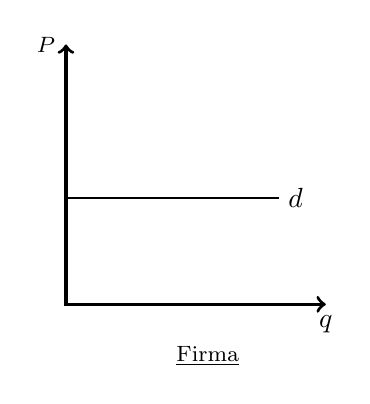
\begin{tikzpicture}[scale=0.3]
\draw[very thick,<->] (0,11) node[left]{\footnotesize $P$}--(0,0)--(11,0) node[below]{$q$};
\draw[thin](0,4.5)--(9,4.5) node [right] {$d$};
\node[] at(6,-2.2) {\footnotesize \underline{Firma}};
\end{tikzpicture}
\end{center}
    \end{minipage}
\end{center}
\end{figure}
\end{center} 
\end{frame}


\begin{frame}
\frametitle{¿Qué pasa en la empresa?}
\begin{figure}[h!]
\centering
\begin{center}
    \begin{minipage}[b]{0.4\textwidth}
    \begin{center}
    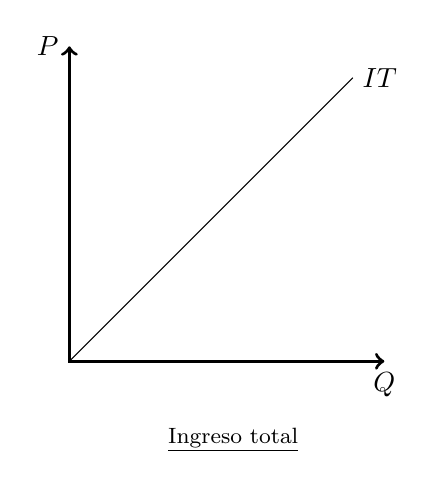
\begin{tikzpicture}[scale=0.4]
\draw[very thick,<->] (0,10) node[left]{$P$}--(0,0)--(10,0) node[below]{$Q$};
%\node [below left] at (0,0) {$0$};
\draw[thin](0,0)--(9,9) node[right] {$IT$};
\node[] at(5.2,-2.5) {\footnotesize \underline{Ingreso total}};
    \end{tikzpicture}
    \end{center}
     \end{minipage}
      \hspace{4mm}
    \begin{minipage}[b]{0.5\textwidth}
    \begin{center}
\begin{tikzpicture}[scale=0.4]
\draw[very thick,<->] (0,10) node[left]{$P$}--(0,0)--(10,0) node[below]{$Q$};
%\node [below left] at (0,0) {$0$};
%\draw[thin, blue](0,5)--(10,5);
\draw[thin](0,5)--(8,5) ;
\node[right] at (8,5){\footnotesize $P = IMg = IMe $};
\node[] at(5.2,-2.5) {\footnotesize \underline{Ingreso marginal y medio}};
\end{tikzpicture}
\end{center}
    \end{minipage}
\end{center}
\end{figure}
\end{frame}

\begin{frame}
\frametitle{¿Qué pasa en la empresa?}
\begin{figure} [h!]
\centering

\tikzset{every picture/.style={line width=0.75pt}} %set default line width to 0.75pt        

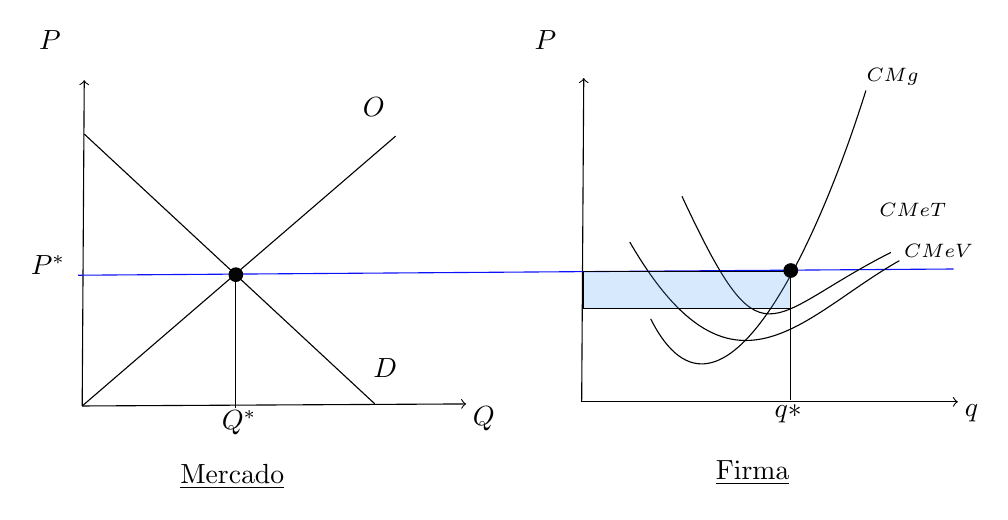
\begin{tikzpicture}[x=0.75pt,y=0.75pt,yscale=-1,xscale=1]
%uncomment if require: \path (0,646); %set diagram left start at 0, and has height of 646

%Straight Lines [id:da47960417398120114] 
\draw    (40,270.69) -- (180,400.69) ;
%Straight Lines [id:da7779767380508746] 
\draw[->]    (39,401.69) -- (39.99,244.69) ;

%Straight Lines [id:da5938498258203935] 
\draw[->]    (39,401.69) -- (224,400.7) ;

%Straight Lines [id:da8399624260742673] 
\draw[->]    (279.65,399.69) -- (460.9,399.69) ;

%Straight Lines [id:da769767421702906] 
\draw[->]    (279.65,399.69) -- (280.65,243.69) ;

%Straight Lines [id:da576259065437712] 
\draw    (39,401.69) -- (190,271.69) ;
%Straight Lines [id:da6704332701835678] 
\draw [color={rgb, 255:red, 11; green, 17; blue, 248 }  ,draw opacity=1 ]   (37,338.69) -- (458.88,335.69) ;
%Curve Lines [id:da29484040262855715] 
\draw    (312.88,359.69) .. controls (347.11,427.69) and (394.44,320.69) .. (416.59,249.69) ;
%Curve Lines [id:da8027323200937775] 
\draw    (302.81,322.69) .. controls (352.15,407.69) and (386.38,357.69) .. (432.7,331.69) ;
%Curve Lines [id:da11645080103937144] 
\draw    (327.98,300.69) .. controls (367.25,384.69) and (367.25,358.69) .. (428.67,327.69) ;
%Straight Lines [id:da9552761772451595] 
\draw    (380.34,354.69) -- (380.34,398.69) ;
%Straight Lines [id:da3598672281312014] 
\draw    (113,341.69) -- (113,402.69) ;
%Shape: Rectangle [id:dp993596205226561] 
\draw   (280.66,336.69) -- (380.34,336.69) -- (380.34,354.69) -- (280.66,354.69) -- cycle ;
%Shape: Rectangle [id:dp396075371323237] 
\draw  [fill={rgb, 255:red, 74; green, 153; blue, 246 }  ,fill opacity=0.22 ] (280.66,336.69) -- (380.34,336.69) -- (380.34,354.69) -- (280.66,354.69) -- cycle ;
%Shape: Circle [id:dp8707642250327381] 
\draw  [fill={rgb, 255:red, 5; green, 5; blue, 5 }  ,fill opacity=1 ] (109.77,338.39) .. controls (109.79,336.58) and (111.27,335.14) .. (113.07,335.16) .. controls (114.88,335.18) and (116.32,336.65) .. (116.3,338.46) .. controls (116.28,340.26) and (114.8,341.71) .. (113,341.69) .. controls (111.2,341.67) and (109.75,340.19) .. (109.77,338.39) -- cycle ;
%Shape: Ellipse [id:dp9369221024836958] 
\draw  [color={rgb, 255:red, 2; green, 2; blue, 2 }  ,draw opacity=1 ][fill={rgb, 255:red, 0; green, 0; blue, 0 }  ,fill opacity=1 ] (377.09,336.39) .. controls (377.11,334.58) and (378.6,333.14) .. (380.41,333.16) .. controls (382.23,333.18) and (383.69,334.65) .. (383.67,336.46) .. controls (383.65,338.26) and (382.16,339.71) .. (380.34,339.69) .. controls (378.53,339.67) and (377.07,338.19) .. (377.09,336.39) -- cycle ;

% Text Node
\draw (17,219.69) node [anchor=north west][inner sep=0.75pt]   [align=left] {$P$};
% Text Node
\draw (226,400.69) node [anchor=north west][inner sep=0.75pt]   [align=left] {$Q$};
% Text Node
\draw (462.96,399.69) node [anchor=north west][inner sep=0.75pt]   [align=left] {$q$};
% Text Node
\draw (255.66,219.69) node [anchor=north west][inner sep=0.75pt]   [align=left] {$P$};
% Text Node
\draw (173,251.69) node [anchor=north west][inner sep=0.75pt]   [align=left] {$O$};
% Text Node
\draw (13,327.69) node [anchor=north west][inner sep=0.75pt]   [align=left] {$P^*$};
% Text Node
\draw (105,402.69) node [anchor=north west][inner sep=0.75pt]   [align=left] {$Q^*$};
% Text Node
\draw (178,377.69) node [anchor=north west][inner sep=0.75pt]   [align=left] {$D$};
% Text Node
\draw (415.71,237.69) node [anchor=north west][inner sep=0.75pt]   [align=left] {\scriptsize $CMg$};
% Text Node
\draw (421.78,302.69) node [anchor=north west][inner sep=0.75pt]   [align=left] {\scriptsize $CMeT$};
% Text Node
\draw (433.79,322.69) node [anchor=north west][inner sep=0.75pt]   [align=left] {\scriptsize $CMeV$};
% Text Node
\draw (371.35,399.69) node [anchor=north west][inner sep=0.75pt]   [align=left] {$q*$};
% Text Node
\draw (85,428.69) node [anchor=north west][inner sep=0.75pt]   [align=left] {\underline{Mercado}};
% Text Node
\draw (343,426.69) node [anchor=north west][inner sep=0.75pt]   [align=left] {\underline{Firma}};
\end{tikzpicture}
\end{figure}
\end{frame}

\begin{frame}
\frametitle{¿Qué pasa si el precio es \textbf{mayor} que el costo marginal?}
\begin{center}
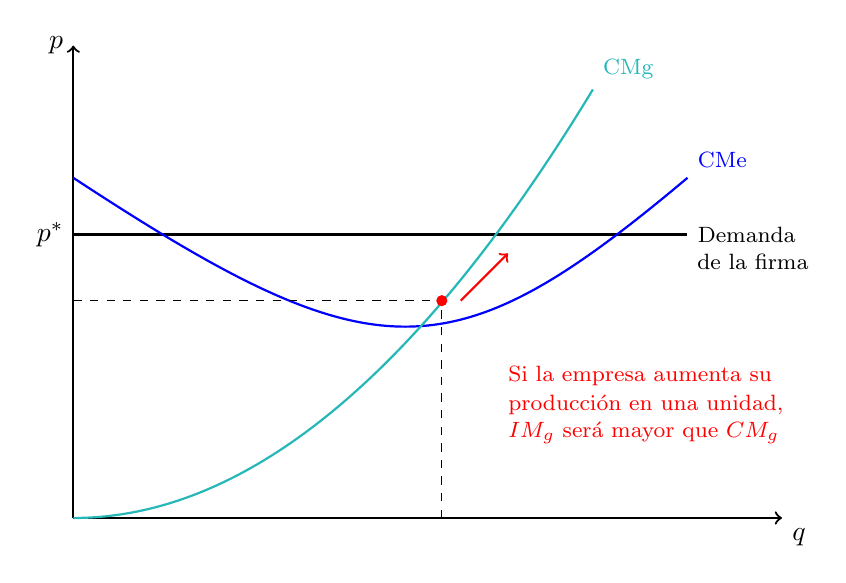
\begin{tikzpicture}[scale=1.2]

% Ejes
\draw[thick, ->] (0,0) -- (7.5,0) node[below right] {$q$};
\draw[thick, ->] (0,0) -- (0,5) node[left] {$p$};

% Línea de precio (demanda perfectamente elástica)
\draw[thick] (0,3) -- (6.5,3) node[right] {\footnotesize Demanda};
\node[below right] at (6.5,2.9) {\footnotesize
  de la firma};

% Costo medio (curva en U)
%\draw[thick, green!70!black] (1.5,4.5)..controls (2.5,2.5) and (3.5,4.5) .. (4.5,5) node[above left] {\scriptsize $CMeT$};

\draw[thick, blue] (0,3.6)..controls (3.2,1.5) and (4,1.5) .. (6.5,3.6)node[above right] {\footnotesize CMe};

% Costo marginal (creciente)
\draw[thick, BlueGreen, domain=0:5.5, samples=100] 
    plot (\x, {0.15*\x^2}) node[above right, BlueGreen] {\footnotesize CMg};

% Línea punteada desde punto de equilibrio
\draw[dashed] (3.9,0) -- (3.9,2.3);
\draw[dashed] (0,2.3) -- (3.9,2.3);

% Punto de intersección
\filldraw[red] (3.9,2.3) circle (1.5pt);

% Etiqueta de p*
\node[left] at (0,3) {$p^*$};

% Flecha azul indicando incentivo a producir más
\draw[->, thick, red] (4.1,2.3) -- (4.6,2.8);

% Texto explicativo
\node[align=left, right, red] at (4.5,1.5) {\footnotesize
  Si la empresa aumenta su};
\node[align=left, right, red] at (4.5,1.2) {\footnotesize
  producción en una unidad,}; 
 \node[align=left, right, red] at (4.5,0.9) {\footnotesize
  $IM_{g}$ será mayor que $CM_{g}$};

\end{tikzpicture}
\end{center}
\end{frame}


\begin{frame}
\frametitle{¿Qué pasa si el precio es \textbf{menor} que el costo marginal?}
\begin{center}
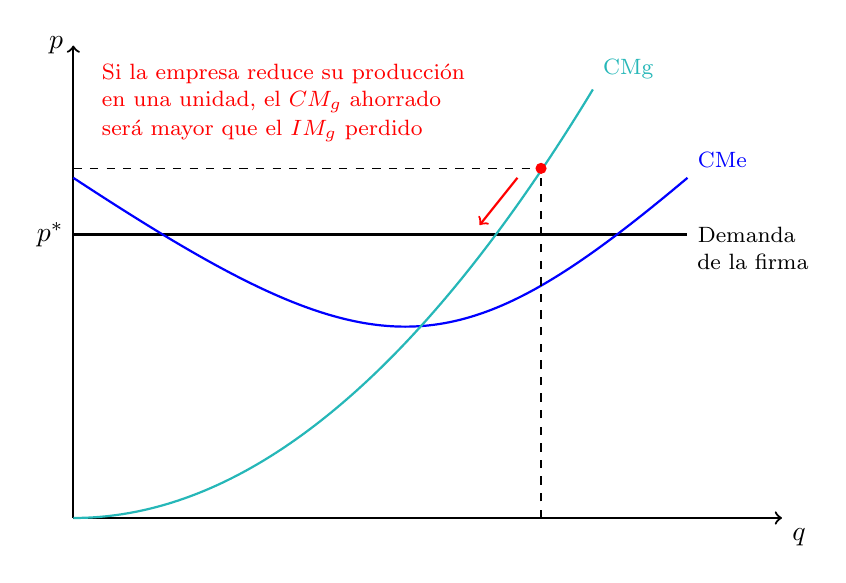
\begin{tikzpicture}[scale=1.2]

% Ejes
\draw[thick, ->] (0,0) -- (7.5,0) node[below right] {$q$};
\draw[thick, ->] (0,0) -- (0,5) node[left] {$p$};

% Línea de precio (demanda perfectamente elástica)
\draw[thick] (0,3) -- (6.5,3) node[right] {\footnotesize Demanda};
\node[below right] at (6.5,2.9) {\footnotesize
  de la firma};

% Costo medio (curva en U)
%\draw[thick, green!70!black] (1.5,4.5)..controls (2.5,2.5) and (3.5,4.5) .. (4.5,5) node[above left] {\scriptsize $CMeT$};

\draw[thick, blue] (0,3.6)..controls (3.2,1.5) and (4,1.5) .. (6.5,3.6)node[above right] {\footnotesize CMe};

% Costo marginal (creciente)
\draw[thick, BlueGreen, domain=0:5.5, samples=100] 
    plot (\x, {0.15*\x^2}) node[above right, BlueGreen] {\footnotesize CMg};

% Línea punteada desde punto de equilibrio
\draw[dashed] (4.95,0) -- (4.95,3.7);
\draw[dashed] (0,3.7) -- (4.95,3.7);

% Punto de intersección
\filldraw[red] (4.95,3.7) circle (1.5pt);

% Etiqueta de p*
\node[left] at (0,3) {$p^*$};

% Flecha 
\draw[->, thick, red] (4.7,3.6) -- (4.3,3.1);

% Texto explicativo
\node[align=left, right, red] at (0.2,4.7) {\footnotesize
  Si la empresa reduce su producción};
\node[align=left, right, red] at (0.2,4.4) {\footnotesize
en una unidad, el $CM_{g}$ ahorrado}; 
 \node[align=left, right, red] at (0.2,4.1) {\footnotesize
   será mayor que el $IM_{g}$ perdido};

\end{tikzpicture}
\end{center}
\end{frame}


%\begin{frame}
%\frametitle{¿Qué pasa si el precio es mayor que el costo marginal?}
%\vspace{3mm}
%\centering
%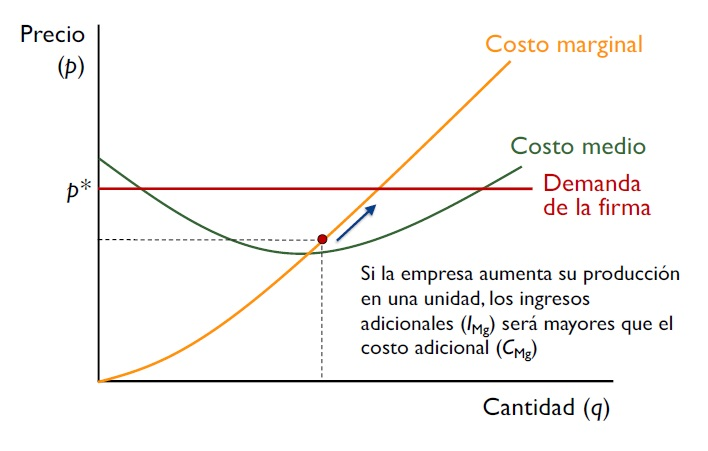
\includegraphics[scale=0.55]{../Figures/Tema_07.8_compperfecta2.jpg}
%\end{frame}

%\begin{frame}
%\frametitle{¿Qué pasa si el precio es menor que el costo marginal?}
%\vspace{3mm}
%\centering
%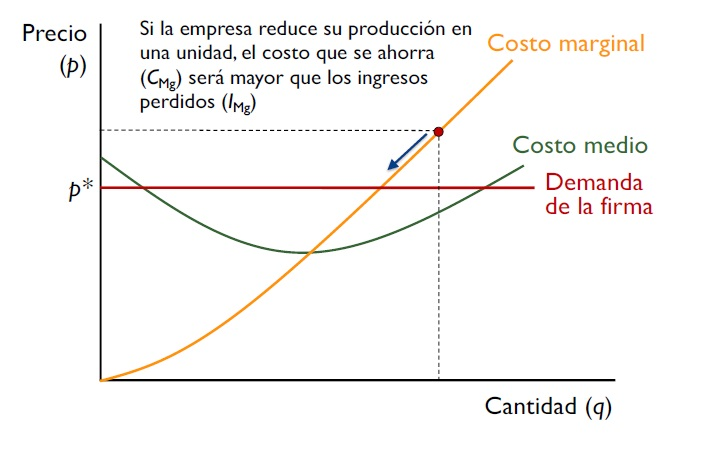
\includegraphics[scale=0.55]{Slides Principios de Economia/Figures/Tema_07.9_compperfecta3.jpg}
%\end{frame}

\begin{frame}
\frametitle{La empresa maximiza beneficios, ¿cómo?}
\begin{center}
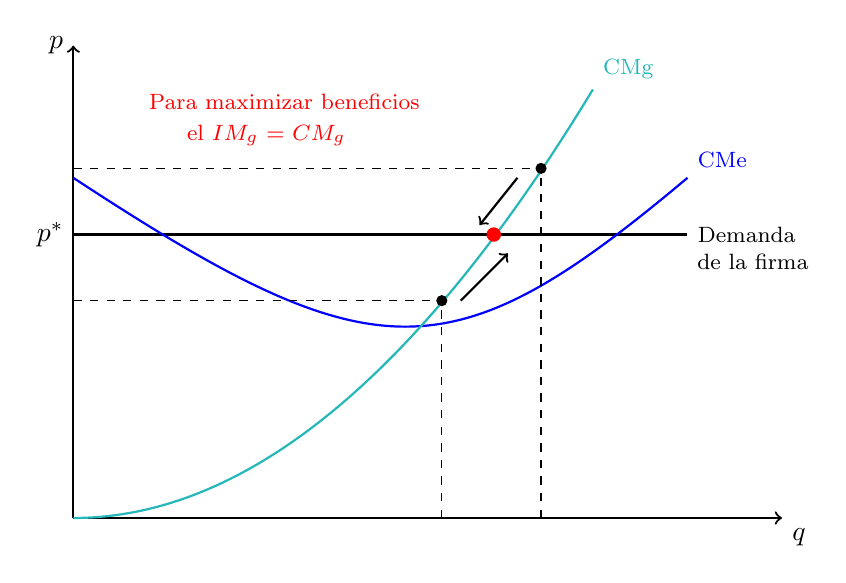
\begin{tikzpicture}[scale=1.2]

% Ejes
\draw[thick, ->] (0,0) -- (7.5,0) node[below right] {$q$};
\draw[thick, ->] (0,0) -- (0,5) node[left] {$p$};

% Línea de precio (demanda perfectamente elástica)
\draw[thick] (0,3) -- (6.5,3) node[right] {\footnotesize Demanda};
\node[below right] at (6.5,2.9) {\footnotesize
  de la firma};

% Costo medio (curva en U)
%\draw[thick, green!70!black] (1.5,4.5)..controls (2.5,2.5) and (3.5,4.5) .. (4.5,5) node[above left] {\scriptsize $CMeT$};

\draw[thick, blue] (0,3.6)..controls (3.2,1.5) and (4,1.5) .. (6.5,3.6)node[above right] {\footnotesize CMe};

% Costo marginal (creciente)
\draw[thick, BlueGreen, domain=0:5.5, samples=100] 
    plot (\x, {0.15*\x^2}) node[above right, BlueGreen] {\footnotesize CMg};
    
% Etiqueta de p*
\node[left] at (0,3) {$p^*$};

% Punto arriba
\draw[dashed] (4.95,0) -- (4.95,3.7);
\draw[dashed] (0,3.7) -- (4.95,3.7);
\filldraw[black] (4.95,3.7) circle (1.5pt);
\draw[->, thick] (4.7,3.6) -- (4.3,3.1);

% Punto abajo
\draw[dashed] (3.9,0) -- (3.9,2.3);
\draw[dashed] (0,2.3) -- (3.9,2.3);
\filldraw[black] (3.9,2.3) circle (1.5pt);
\draw[->, thick] (4.1,2.3) -- (4.6,2.8);

\filldraw[red] (4.45,3) circle (2pt);
\node[align=left, right, red] at (0.7,4.4) {\footnotesize
  Para maximizar beneficios};
\node[align=left, right, red] at (1.1,4.05) {\footnotesize
el $IM_{g}$ = $CM_{g}$}; 

\end{tikzpicture}
\end{center}
\end{frame}

%\begin{frame}
%\frametitle{Veamos un ejemplo}
%\begin{itemize}
%    \item Precio: \$32
%    \item Costo marginal = $2Q^{2}$
%\end{itemize}
%\begin{table}[h]
%    \centering
%    \renewcommand{\arraystretch}{1.3} % Espaciado entre filas
%    \setlength{\tabcolsep}{8pt} % Espaciado entre columnas
%    \rowcolors{2}{white!100}{white!95} % Alternar colores de filas
%    \newcolumntype{P}{>{\centering\arraybackslash}p{1.4cm}}
%    \begin{tabular}{|P|P|P|P|P|P|}
%        \hline
%        \rowcolor{blue!20} % Color de fondo del encabezado
%        Q & P (IMg)  & CMg & CT & IT & Beneficio \\
%        \hline
%        0 & 32 &   &   &    &    \\
%        1 & 32 &   &    &    &    \\
%        2 & 32 &   &    &    &   \\
%        3 & 32 &   &    &    &    \\
%        4 & 32 &   &    &    &    \\
%        5 & 32 &  &    &    &     \\
%        \hline
%    \end{tabular}
%\end{table}
%\end{frame}

%\begin{frame}
%\frametitle{Veamos un ejemplo}
%\begin{itemize}
%    \item Precio: \$32
%    \item Costo marginal = $2Q^{2}$
%\end{itemize}
%\begin{table}[h]
%    \centering
%    \renewcommand{\arraystretch}{1.3} % Espaciado entre filas
%    \setlength{\tabcolsep}{8pt} % Espaciado entre columnas
%    \rowcolors{2}{white!100}{white!95} % Alternar colores de filas
%    \newcolumntype{P}{>{\centering\arraybackslash}p{1.4cm}}
%    \begin{tabular}{|P|P|P|P|P|P|}
%        \hline
%        \rowcolor{blue!20} % Color de fondo del encabezado
%        Q & P (IMg)  & CMg & CT & IT & Beneficio \\
%        \hline
%        0 & 32 &  0 &  0 &  0  &   0 \\
%        1 & 32 &  2 &  2  &  32  &  30  \\
%        2 & 32 &  8 &  10  &  64  &  54 \\
%        3 & 32 &  18 &  28  &  96  &  68  \\
%        4 & 32 &  32 &  60  &  128  &  68  \\
%        5 & 32 & 50 &  110  &  160  &   50  \\
%        \hline
%    \end{tabular}
%\end{table}
%\end{frame}

\begin{frame}
\frametitle{Veamos un ejemplo}
\begin{itemize}
    \item Supongamos que una empresa enfrenta un precio: P= \$6
\end{itemize}
\begin{table}[h]
    \centering
    \renewcommand{\arraystretch}{1.3} % Espaciado entre filas
    \setlength{\tabcolsep}{6pt} % Espaciado entre columnas
    \rowcolors{2}{white!100}{white!95} % Alternar colores de filas
    \newcolumntype{P}{>{\centering\arraybackslash}p{1.25cm}}
    \begin{tabular}{|P|P|P|P|P|P|P|}
        \hline
        \rowcolor{blue!20} % Color de fondo del encabezado
        Q & IT  & CT & IMg & CMg & Beneficio & BMg\\
        \hline
        0 &   &  3 &   &    &  &  \\
        1 &   &  5 &   &    &   &  \\
        2 &  &  8 &    &    &   &  \\
        3 &  &  12 &    &   &   &  \\
        4 &  &  17 &   &   &  &  \\
        5 &  &  23 &    &   &  &  \\
        6 &  & 30 &   &   &  &  \\
        7 &  & 38 &    &   &   & \\

        \hline
    \end{tabular}
\end{table}
\end{frame}

\begin{frame}
\frametitle{Veamos un ejemplo}
\begin{itemize}
    \item Supongamos que una empresa enfrenta un precio: P= \$6
\end{itemize}
\begin{table}[h]
    \centering
    \renewcommand{\arraystretch}{1.3} % Espaciado entre filas
    \setlength{\tabcolsep}{6pt} % Espaciado entre columnas
    \rowcolors{2}{white!100}{white!95} % Alternar colores de filas
    \newcolumntype{P}{>{\centering\arraybackslash}p{1.25cm}}
    \begin{tabular}{|P|P|P|P|P|P|P|}
        \hline
        \rowcolor{blue!20} % Color de fondo del encabezado
        Q & IT  & CT & IMg & CMg & Beneficio & BMg\\
        \hline
        0 &  0 &  3 &   &    & -3 &  \\
        1 &  6 &  5 &  6 &  2  &  1 & 1 \\
        2 & 12 &  8 &  6  &  3  &  4 & 3 \\
        3 & 18 &  12 &  6  &  4  &  6 & 2 \\
        4 & 24 &  17 & 6  &  5  &  7 & 1 \\
        5 & 30 &  23 &  6  &  6  & 7  & 0 \\
        6 & 36 & 30 & 6  &  7  &  6 & -1 \\
        7 & 42 & 38 &  6  &  8  &  4  &-2 \\

        \hline
    \end{tabular}
\end{table}
\end{frame}

\begin{frame}
\frametitle{¿Hay beneficio en este punto? SI!}
\begin{center}
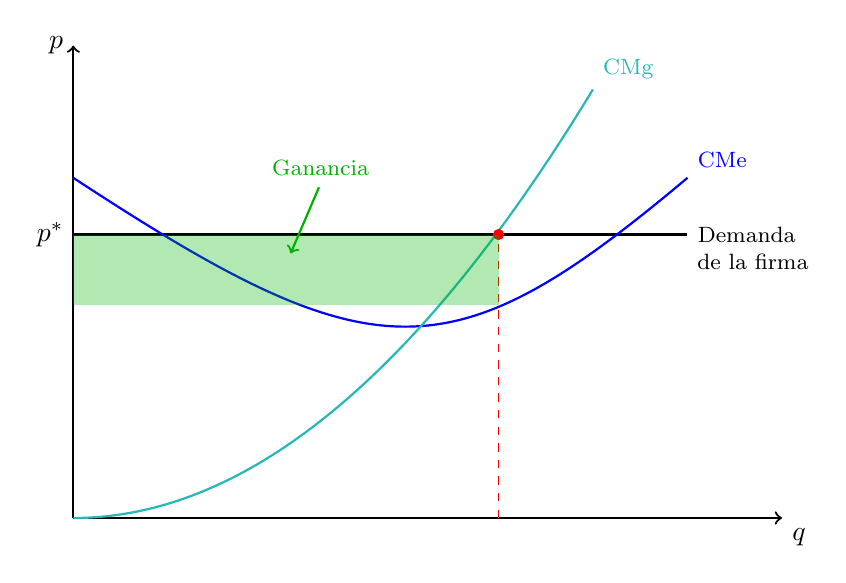
\begin{tikzpicture}[scale=1.2]

% Ejes
\draw[thick, ->] (0,0) -- (7.5,0) node[below right] {$q$};
\draw[thick, ->] (0,0) -- (0,5) node[left] {$p$};

% Línea de precio (demanda perfectamente elástica)
\draw[thick] (0,3) -- (6.5,3) node[right] {\footnotesize Demanda};
\node[below right] at (6.5,2.9) {\footnotesize
  de la firma};

\draw[thick, blue] (0,3.6)..controls (3.2,1.5) and (4,1.5) .. (6.5,3.6)node[above right] {\footnotesize CMe};

\draw[thick, BlueGreen, domain=0:5.5, samples=100] 
    plot (\x, {0.15*\x^2}) node[above right, BlueGreen] {\footnotesize CMg};

% Línea punteada desde punto de equilibrio
\draw[dashed, red] (4.5,0) -- (4.5,3);

% Punto de intersección
\filldraw[red] (4.5,3) circle (1.5pt);
\node[left] at (0,3) {$p^*$};

\fill[green!70!black, opacity=0.3] (0,2.25) rectangle (4.5,3);

\draw[->, thick, green!70!black] (2.6,3.5) -- (2.3,2.8);
 \node[align=left, right, green!70!black] at (2,3.7) {\footnotesize
   Ganancia};

\end{tikzpicture}
\end{center}
\end{frame}


%\begin{frame}
%\frametitle{¿Habrá beneficio en este punto? SI!}
%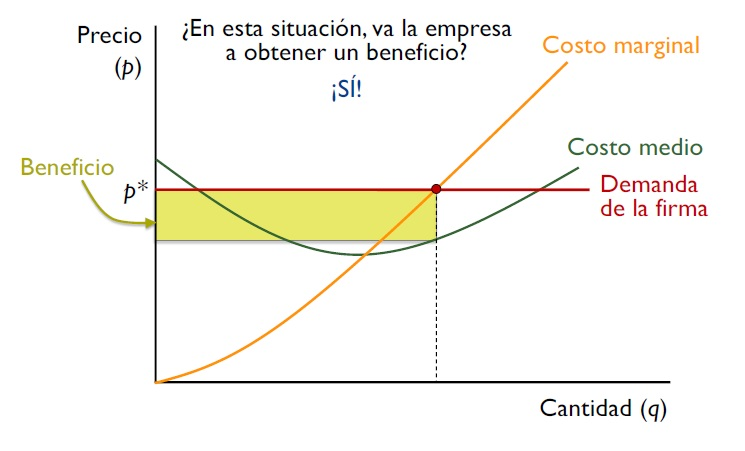
\includegraphics[scale=0.55]{Slides Principios de Economia/Figures/Tema_07.11_compperfecta5.jpg}
%\end{frame}

\begin{frame}
\frametitle{¿Hay beneficio en este punto? NO! Pero sí hay pérdida}
\begin{center}
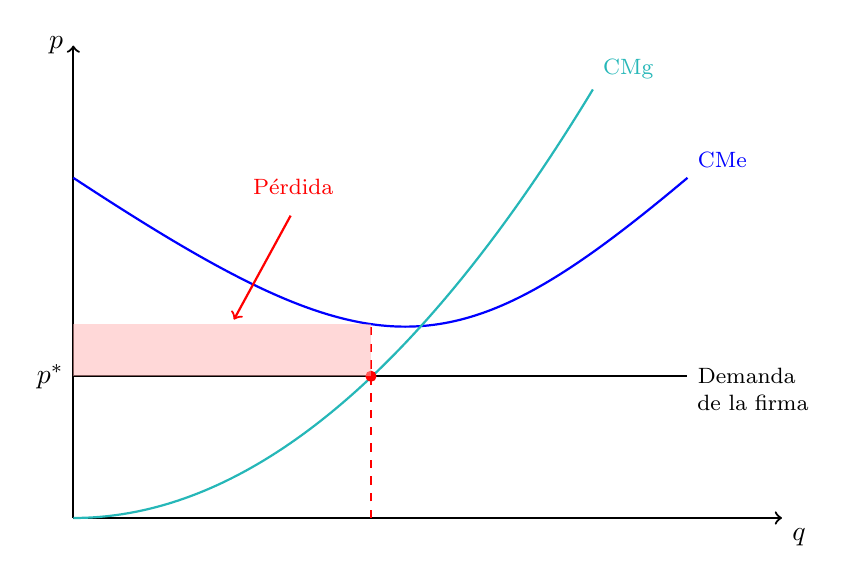
\begin{tikzpicture}[scale=1.2]

% Ejes
\draw[thick, ->] (0,0) -- (7.5,0) node[below right] {$q$};
\draw[thick, ->] (0,0) -- (0,5) node[left] {$p$};

% Línea de precio (demanda perfectamente elástica)
\draw[thick] (0,1.5) -- (6.5,1.5) node[right] {\footnotesize Demanda};
\node[below right] at (6.5,1.4) {\footnotesize
  de la firma};

\draw[thick, blue] (0,3.6)..controls (3.2,1.5) and (4,1.5) .. (6.5,3.6)node[above right] {\footnotesize CMe};

\draw[thick, BlueGreen, domain=0:5.5, samples=100] 
    plot (\x, {0.15*\x^2}) node[above right, BlueGreen] {\footnotesize CMg};

% Línea punteada desde punto de equilibrio
\draw[dashed, red] (3.15,0) -- (3.15,2.05);

% Punto de intersección
\filldraw[red] (3.15,1.5) circle (1.5pt);
\node[left] at (0,1.5) {$p^*$};

\fill[red!30, opacity=0.5] (0,1.5) rectangle (3.15,2.05);

\draw[->, thick, red] (2.3,3.2) -- (1.7,2.1);
 \node[align=left, right, red] at (1.8,3.5) {\footnotesize
   Pérdida};
   
\end{tikzpicture}
\end{center}
\end{frame}

%\begin{frame}
%\frametitle{¿Habrá beneficio en este punto? NO! ¿Hay perdida? SI!}
%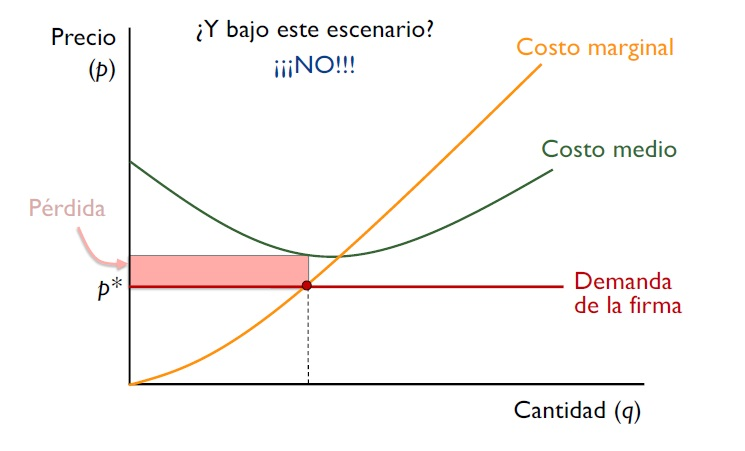
\includegraphics[scale=0.55]{Slides Principios de Economia/Figures/Tema_07.12_compperfecta6.jpg}
%\end{frame}

\begin{frame}
\frametitle{Ni ganancia ni pérdida}
\begin{center}
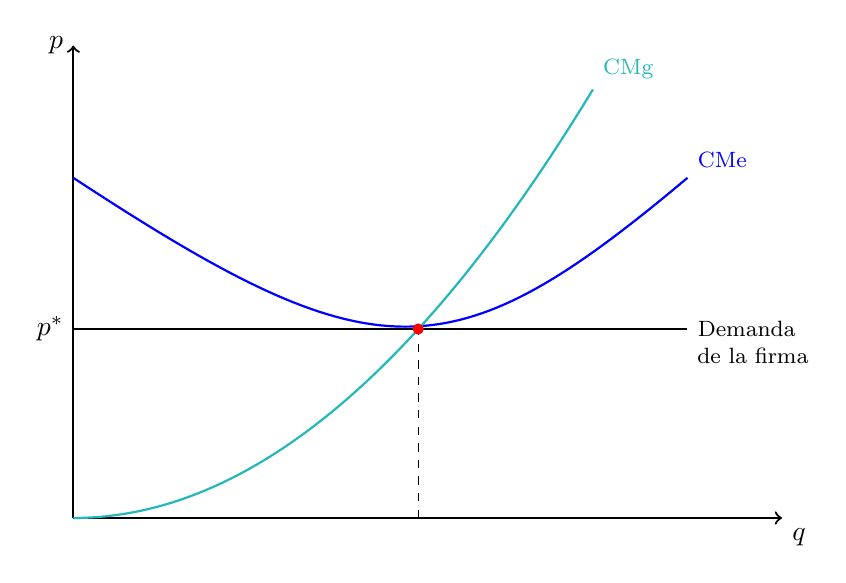
\begin{tikzpicture}[scale=1.2]

% Ejes
\draw[thick, ->] (0,0) -- (7.5,0) node[below right] {$q$};
\draw[thick, ->] (0,0) -- (0,5) node[left] {$p$};

% Línea de precio (demanda perfectamente elástica)
\draw[thick] (0,2) -- (6.5,2) node[right] {\footnotesize Demanda};
\node[below right] at (6.5,1.9) {\footnotesize
  de la firma};

\draw[thick, blue] (0,3.6)..controls (3.2,1.5) and (4,1.5) .. (6.5,3.6)node[above right] {\footnotesize CMe};

\draw[thick, BlueGreen, domain=0:5.5, samples=100] 
    plot (\x, {0.15*\x^2}) node[above right, BlueGreen] {\footnotesize CMg};

% Línea punteada desde punto de equilibrio
\draw[dashed] (3.65,0) -- (3.65,2);

% Punto de intersección
\filldraw[red] (3.65,2) circle (1.5pt);
\node[left] at (0,2) {$p^*$};


\end{tikzpicture}
\end{center}
\end{frame}


%\begin{frame}
%\frametitle{¿Habrá beneficio extraordinario en este punto? NO! ¿Hay perdida? NO!}
%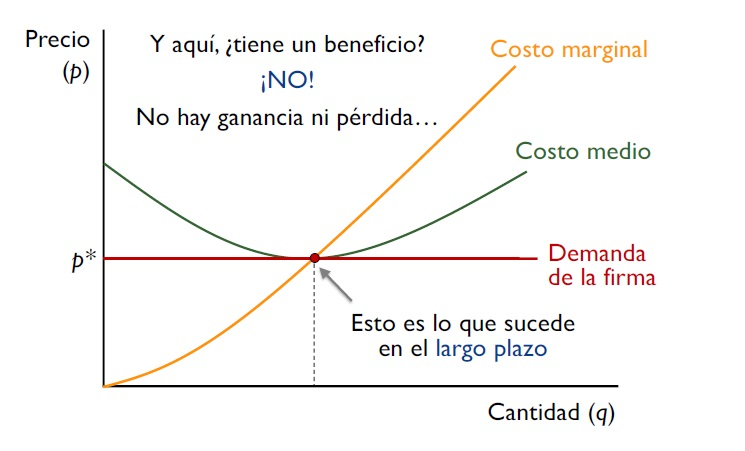
\includegraphics[scale=0.55]{Slides Principios de Economia/Figures/Tema_07.13_compperfecta7.jpg}
%\end{frame}

\begin{frame}
    \frametitle{En el corto plazo - maximizar beneficios}
\begin{itemize}
    \item   \textbf{En competencia perfecta}, \textbf{la empresa maximiza sus beneficios} en el corto plazo cuando el ingreso marginal se iguala al costo marginal. Es decir, \textbf{cuando el precio se iguala al costo marginal.} \vspace{2mm}
    \item Pero ojo, produce \textbf{solo si el precio} (que observa en el mercadp) \textbf{supera el costo medio variable en el punto donde maximiza sus beneficios}.
\end{itemize}
\end{frame}

\begin{frame}
    \frametitle{En el corto plazo -  cierre}
\begin{itemize}
    \item  Dado que en el corto plazo las empresas no pueden evitar los costos fijos, cerrará ($Q=0$) si el ingreso que obtendría de producir es menor que los costos variables de la producción: 
            \[ IT< CV \]
Lo que es lo mismo que:
\[ \frac{IT}{Q} < \frac{CV}{Q} \]
Como en competencia perfecta $IMe=P$, 
\[ P < CVMe \]
\item Es decir, si el precio no cubre el $CVMe$, la empresa estará mejor si deja de producir por completo. Pierde dinero de todos modos (porque tiene que pagar los costos fijos), pero perdería más si sigue operando.
\end{itemize}
\end{frame}

\begin{frame}
\frametitle{¿Y en el largo plazo...?}
\begin{itemize}
\item Los beneficios extraordinarios son las ganancias de corto plazo que reciben las empresas en competencia perfecta.
    \begin{itemize}
    \item Se trata de la rentabilidad que obtienen la empresas por encima de la tasa de retorno normal (que considera todos los costos relevantes, \underline{incluyendo el costo de oportunidad del capital}).
    \end{itemize}
    \item Siempre que existan potenciales rentas (beneficios extraordinarios), va a haber firmas interesadas en entrar al mercado
    \item Si los costos de entrada no son demasiado altos, estas firmas potenciales van a entrar
    \item Al ingresar, las firmas van a presionar hacia abajo el precio de equilibrio, eliminando del mercado a las firmas menos eficientes
    \item Los beneficios que atraen a potenciales entrantes comienzan a disiparse
    \item En el largo plazo, estos beneficios van a desaparecer, serán iguales a 0.
    \end{itemize}
\end{frame}

\begin{frame}
\frametitle{¿Y en el largo plazo...?}
\begin{center}
\begin{figure} [H]
\centering
\tikzset{every picture/.style={line width=0.75pt}} %set default line width to 0.75pt        

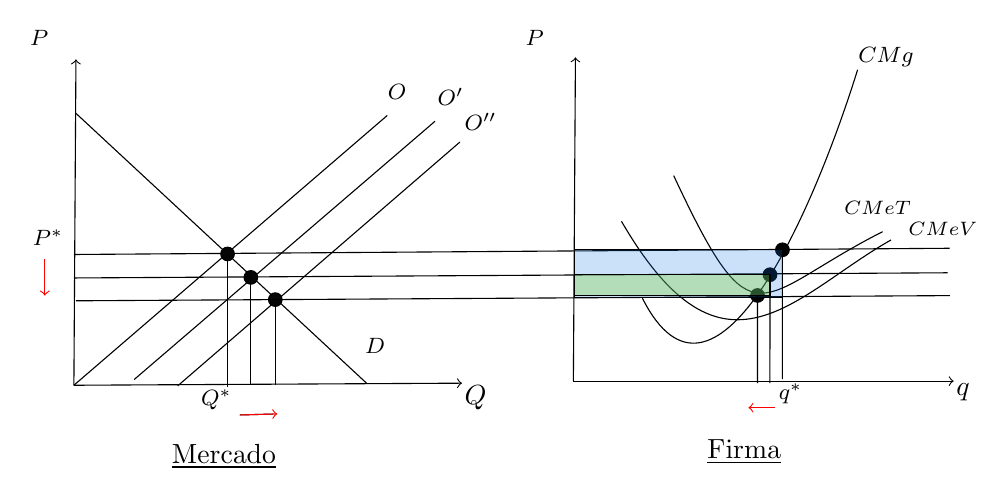
\begin{tikzpicture}[x=0.75pt,y=0.75pt,yscale=-1,xscale=1] [scale=0.8]
%uncomment if require: \path (0,2084); %set diagram left start at 0, and has height of 2084

%Straight Lines [id:da060960642870382165] 
\draw    (76,1041.69) -- (216,1171.69) ;
%Straight Lines [id:da7851707797387746] 
\draw[->] (75,1172.69) -- (75.99,1015.69);
%Straight Lines [id:da5252533350679736] 
\draw[->] (75,1172.69) -- (262,1171.69);
%Straight Lines [id:da1925274721555612] 
\draw    (315.65,1170.69) -- (496.9,1170.69) ;
%Straight Lines [id:da06122585785191381] 
\draw[->]    (315.65,1170.69) -- (316.65,1014.69) ;
\draw[->] (315.65,1170.69) -- (498.9,1170.69);
%Straight Lines [id:da431398071619699] 
\draw    (75,1172.69) -- (226,1042.69) ;
%Straight Lines [id:da6076203558210751] 
\draw [color={rgb, 255:red, 0; green, 0; blue, 0 }  ,draw opacity=1 ]   (75,1109.69) -- (496.88,1106.69) ;
%Curve Lines [id:da8172716073565294] 
\draw    (348.88,1130.69) .. controls (383.11,1198.69) and (430.44,1091.69) .. (452.59,1020.69) ;
%Curve Lines [id:da7210609848314191] 
\draw    (338.81,1093.69) .. controls (388.15,1178.69) and (422.38,1128.69) .. (468.7,1102.69) ;
%Curve Lines [id:da02485638109474686] 
\draw    (363.98,1071.69) .. controls (403.25,1155.69) and (403.25,1129.69) .. (464.67,1098.69) ;
%Straight Lines [id:da9738419389002844] 
\draw    (416.38,1107.42) -- (416.34,1169.69) ;
%Straight Lines [id:da17644987359180853] 
\draw    (149,1112.69) -- (149,1173.69) ;
%Shape: Circle [id:dp2973355629068237] 
\draw  [fill={rgb, 255:red, 5; green, 5; blue, 5 }  ,fill opacity=1 ] (145.77,1109.39) .. controls (145.79,1107.58) and (147.27,1106.14) .. (149.07,1106.16) .. controls (150.88,1106.18) and (152.32,1107.65) .. (152.3,1109.46) .. controls (152.28,1111.26) and (150.8,1112.71) .. (149,1112.69) .. controls (147.2,1112.67) and (145.75,1111.19) .. (145.77,1109.39) -- cycle ;
%Shape: Ellipse [id:dp8539925560604675] 
\draw  [color={rgb, 255:red, 2; green, 2; blue, 2 }  ,draw opacity=1 ][fill={rgb, 255:red, 0; green, 0; blue, 0 }  ,fill opacity=1 ] (413.09,1107.39) .. controls (413.11,1105.58) and (414.6,1104.14) .. (416.41,1104.16) .. controls (418.23,1104.18) and (419.69,1105.65) .. (419.67,1107.46) .. controls (419.65,1109.26) and (418.16,1110.71) .. (416.34,1110.69) .. controls (414.53,1110.67) and (413.07,1109.19) .. (413.09,1107.39) -- cycle ;
%Straight Lines [id:da14289261334513892] 
\draw    (104.07,1169.91) -- (249,1045.5) ;
%Straight Lines [id:da31165236436665356] 
\draw    (75,1121) -- (496,1118.5) ;
%Shape: Circle [id:dp9941417879817387] 
\draw  [fill={rgb, 255:red, 5; green, 5; blue, 5 }  ,fill opacity=1 ] (157,1120.69) .. controls (157.02,1118.88) and (158.5,1117.44) .. (160.3,1117.46) .. controls (162.11,1117.48) and (163.55,1118.96) .. (163.53,1120.76) .. controls (163.51,1122.56) and (162.03,1124.01) .. (160.23,1123.99) .. controls (158.43,1123.97) and (156.98,1122.49) .. (157,1120.69) -- cycle ;
%Straight Lines [id:da7694650098831262] 
\draw    (160,1118.69) -- (160,1172.5) ;
%Straight Lines [id:da5710733904002603] 
\draw    (61,1112) -- (61,1127.5) ;
\draw[->, red] (61,1112) -- (61,1129.5);
%Straight Lines [id:da30346292560316446] 
\draw    (125,1173) -- (261,1055.5) ;
%Shape: Circle [id:dp9338937817809183] 
\draw  [fill={rgb, 255:red, 5; green, 5; blue, 5 }  ,fill opacity=1 ] (168.77,1131.39) .. controls (168.79,1129.58) and (170.27,1128.14) .. (172.07,1128.16) .. controls (173.88,1128.18) and (175.32,1129.65) .. (175.3,1131.46) .. controls (175.28,1133.26) and (173.8,1134.71) .. (172,1134.69) .. controls (170.2,1134.67) and (168.75,1133.19) .. (168.77,1131.39) -- cycle ;
%Straight Lines [id:da9716189952078933] 
\draw    (76,1132) -- (497,1129.5) ;
%Straight Lines [id:da7462100456158596] 
\draw    (172,1134.69) -- (172,1172.5) ;
%Straight Lines [id:da6840836726821611] 
\draw    (155,1187) -- (171,1186.56) ;
\draw[->, red] (155,1187) -- (173,1186.5);
%Straight Lines [id:da7200406093384826] 
\draw[->, red]    (413,1183.5) -- (400,1183.5) ;

%Shape: Ellipse [id:dp4431909589126928] 
\draw  [color={rgb, 255:red, 2; green, 2; blue, 2 }  ,draw opacity=1 ][fill={rgb, 255:red, 0; green, 0; blue, 0 }  ,fill opacity=1 ] (407.09,1119.39) .. controls (407.11,1117.58) and (408.6,1116.14) .. (410.41,1116.16) .. controls (412.23,1116.18) and (413.69,1117.65) .. (413.67,1119.46) .. controls (413.65,1121.26) and (412.16,1122.71) .. (410.34,1122.69) .. controls (408.53,1122.67) and (407.07,1121.19) .. (407.09,1119.39) -- cycle ;
%Shape: Ellipse [id:dp8179688386007129] 
\draw  [color={rgb, 255:red, 2; green, 2; blue, 2 }  ,draw opacity=1 ][fill={rgb, 255:red, 0; green, 0; blue, 0 }  ,fill opacity=1 ] (401.09,1129.39) .. controls (401.11,1127.58) and (402.6,1126.14) .. (404.41,1126.16) .. controls (406.23,1126.18) and (407.69,1127.65) .. (407.67,1129.46) .. controls (407.65,1131.26) and (406.16,1132.71) .. (404.34,1132.69) .. controls (402.53,1132.67) and (401.07,1131.19) .. (401.09,1129.39) -- cycle ;
%Shape: Rectangle [id:dp583804092155076] 
\draw  [fill={rgb, 255:red, 18; green, 117; blue, 234 }  ,fill opacity=0.22 ] (316,1107.42) -- (416.38,1107.42) -- (416.38,1130.5) -- (316,1130.5) -- cycle ;
%Shape: Rectangle [id:dp5629735949679284] 
\draw  [fill={rgb, 255:red, 126; green, 211; blue, 33 }  ,fill opacity=0.3 ] (316,1119.42) -- (410.38,1119.42) -- (410.38,1129.46) -- (316,1129.46) -- cycle ;
%Straight Lines [id:da14635641253383858] 
\draw    (410.38,1129.42) -- (410.34,1171.69) ;
%Straight Lines [id:da9761281060467815] 
\draw    (404.38,1129.42) -- (404.34,1171.69) ;

% Text Node
\draw (53,1000.69) node [anchor=north west][inner sep=0.5pt]   [align=left] {\footnotesize $P$};
% Text Node
\draw (262,1171.69) node [anchor=north west][inner sep=0.75pt]   [align=left] {$Q$};
% Text Node
\draw (498.96,1170.69) node [anchor=north west][inner sep=0.75pt]   [align=left] {$q$};
% Text Node
\draw (291.66,1000.69) node [anchor=north west][inner sep=0.5pt]   [align=left] {\footnotesize $P$};
% Text Node
\draw (225,1026.69) node [anchor=north west][inner sep=0.75pt]  [font=\footnotesize] [align=left] {\footnotesize $O$};
% Text Node
\draw (54,1096.69) node [anchor=north west][inner sep=0.75pt]  [font=\footnotesize] [align=left] {\footnotesize $P^*$};
% Text Node
\draw (135,1173.69) node [anchor=north west][inner sep=0.75pt]   [align=left] {\footnotesize $Q^*$};
% Text Node
\draw (214,1148.69) node [anchor=north west][inner sep=0.75pt]   [align=left] {\footnotesize $D$};
% Text Node
\draw (451.71,1008.69) node [anchor=north west][inner sep=0.75pt]   [align=left] {\footnotesize $CMg$};
% Text Node
\draw (444.78,1082.69) node [anchor=north west][inner sep=0.75pt]   [align=left] {\scriptsize $CMeT$};
% Text Node
\draw (475.79,1092.69) node [anchor=north west][inner sep=0.75pt]   [align=left] {\scriptsize $CMeV$};
% Text Node
\draw (413.35,1170.69) node [anchor=north west][inner sep=0.75pt]   [align=left] {\footnotesize $q^*$};
% Text Node
\draw (121,1199.69) node [anchor=north west][inner sep=0.75pt]   [align=left] {\underline{Mercado}};
% Text Node
\draw (379,1197.69) node [anchor=north west][inner sep=0.75pt]   [align=left] {\underline{Firma}};
% Text Node
\draw (249,1028.5) node [anchor=north west][inner sep=0.75pt]  [font=\footnotesize] [align=left] {\footnotesize $O'$};
% Text Node
\draw (262,1040.5) node [anchor=north west][inner sep=0.75pt]  [font=\footnotesize] [align=left] {\footnotesize $O''$};
\end{tikzpicture}
\end{figure}
\end{center}
\end{frame}

\begin{frame}
\frametitle{¿Y en el largo plazo...?}
\begin{figure}[h]
\tikzset{every picture/.style={line width=0.75pt}} %set default line width to 0.75pt        

\begin{tikzpicture}[x=0.75pt,y=0.75pt,yscale=-1,xscale=1] 
%uncomment if require: \path (0,1657); %set diagram left start at 0, and has height of 1657

%Straight Lines [id:da6123979361342768] 
\draw[->]     (74,298) -- (344,298) ;
%Straight Lines [id:da5131707791527922] 
\draw[->]    (74,298) -- (74,48) ;
%Straight Lines [id:da6346804843028921] 
\draw    (75,188) -- (334,189) ;
%Curve Lines [id:da697350144213293] 
\draw    (109,126) .. controls (142,212) and (270,204) .. (297,123) ;
%Curve Lines [id:da9799910224345574] 
\draw    (112,229) .. controls (136,295) and (246,141) .. (271,95) ;
%Straight Lines [id:da5845279516726063] 
\draw    (204.5,188.5) -- (204,297) ;

% Text Node
\draw (45,35) node [anchor=north west][inner sep=0.5pt]   [align=left] {$P$};
% Text Node
\draw (346,298) node [anchor=north west][inner sep=0.75pt]   [align=left] {$q$};
% Text Node
\draw (297,123) node [anchor=north west][inner sep=0.75pt]   [align=left] {$CMeT$};
% Text Node
\draw (271,85) node [anchor=north west][inner sep=0.75pt]   [align=left] {$CMg$};
% Text Node
\draw (50,178) node [anchor=north west][inner sep=0.75pt]   [align=left] {$P^*$};
% Text Node
\draw (194,299) node [anchor=north west][inner sep=0.75pt]   [align=left] {$q^*$};
\end{tikzpicture}
\end{figure}
\end{frame}

\begin{frame}
\frametitle{¿Y en el largo plazo...?}
\begin{itemize}
    \item Vimos que en el equilibrio a largo plazo, el precio $P$ es igual al costo marginal $CMg$, por lo que la empresa maximiza sus beneficios. El precio también es igual al costo total promedio $CTMe$, por lo que los beneficios son cero.
    \item ¿Qué implica esto? Que las empresas en el largo plazo operan en su escala eficiente!
    \item Recuerden que el $CMg$ se iguala con el $CTMe$  solo cuando la empresa opera en el mínimo de su costo total promedio.
\end{itemize}



\end{frame}

\begin{frame}
\frametitle{¿Por qué es eficiente?}
\begin{itemize}
    \item Los participantes son tomadores de precios
    \begin{itemize}
        \item No hay poder de mercado.
        \item La competencia impide a los vendedores aumentar el precio, y a los compradores bajarlo.
    \end{itemize}
    \item No hay barreras de entrada
    \item Los contratos son completos
        \begin{itemize}
        \item Los detalles del intercambio pueden ser definidos en forma clara, y estos contratos se pueden hacer cumplir.
        \end{itemize}
    \item No hay externalidades
        \begin{itemize}
        \item La transacción sólo afecta a los compradores y vendedores
        \end{itemize}
\end{itemize}
\end{frame}

\begin{frame}
\frametitle{Conclusión de largo plazo}

\begin{itemize}
\item ¿Por qué las empresas competitivas siguen operando si obtienen cero beneficios?
\item Recuerden la distinción entre beneficios contables y beneficios económicos. Estos últimos incluyen todos los costos de oportunidad de la empresa.
\item En el equilibrio de cero beneficios, los ingresos de la empresa deben compensar a los propietarios por estos costos de oportunidad.

\end{itemize}
\end{frame}


\end{document}
